\subsectionaddtolist{فهم اولیه از HTTP}

ابتدا نرم‌‌افزار Wireshark را باز کرده و روی حالت capture قرار می‌دهیم،
سپس وب‌سایت 
\lr{https://uranus-agency.ir/gallery/}
را باز می‌کنیم. در نهایت capture را متوقف می‌کنیم و پکت‌ها را مشاهده می‌کنیم:

{
	\centering{
		
		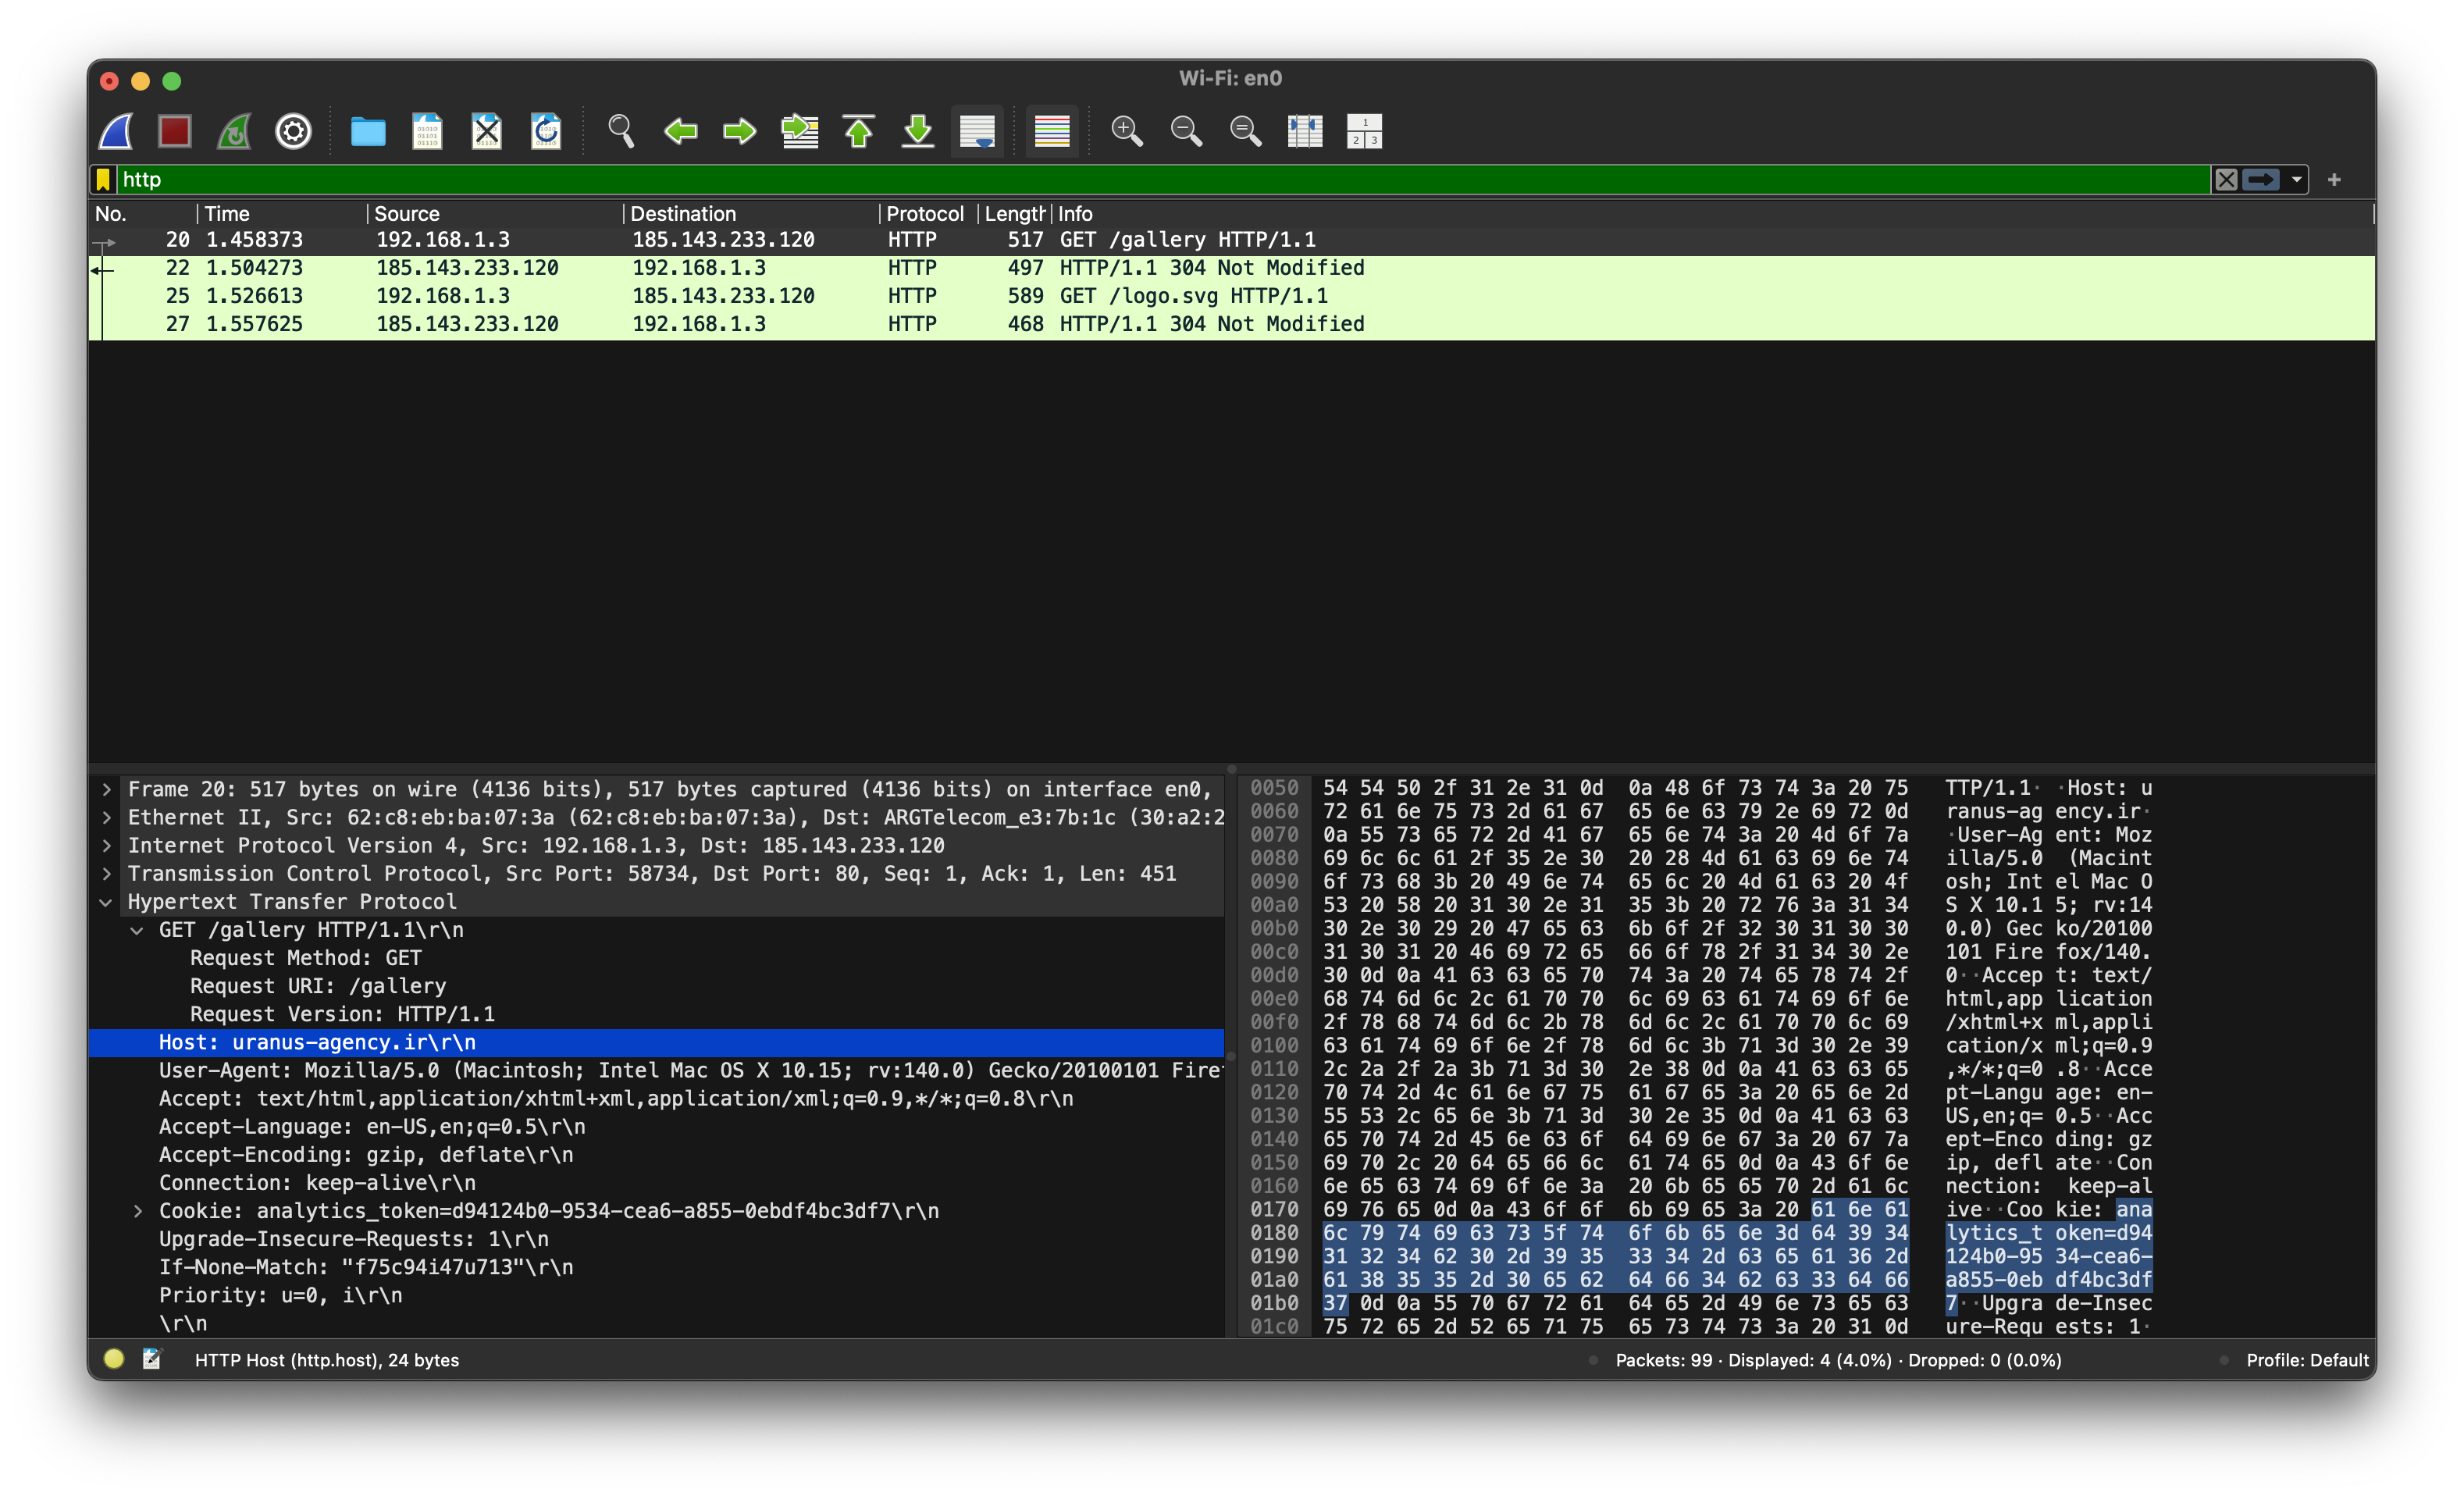
\includegraphics[width=1\textwidth]{figs/1.png}
		
	}
}


\subsubsection*{سوال ۱.}

از گزینه statistics بر روی protocol-hierarchy کلیک می‌کنیم.


{
	\centering{
		
		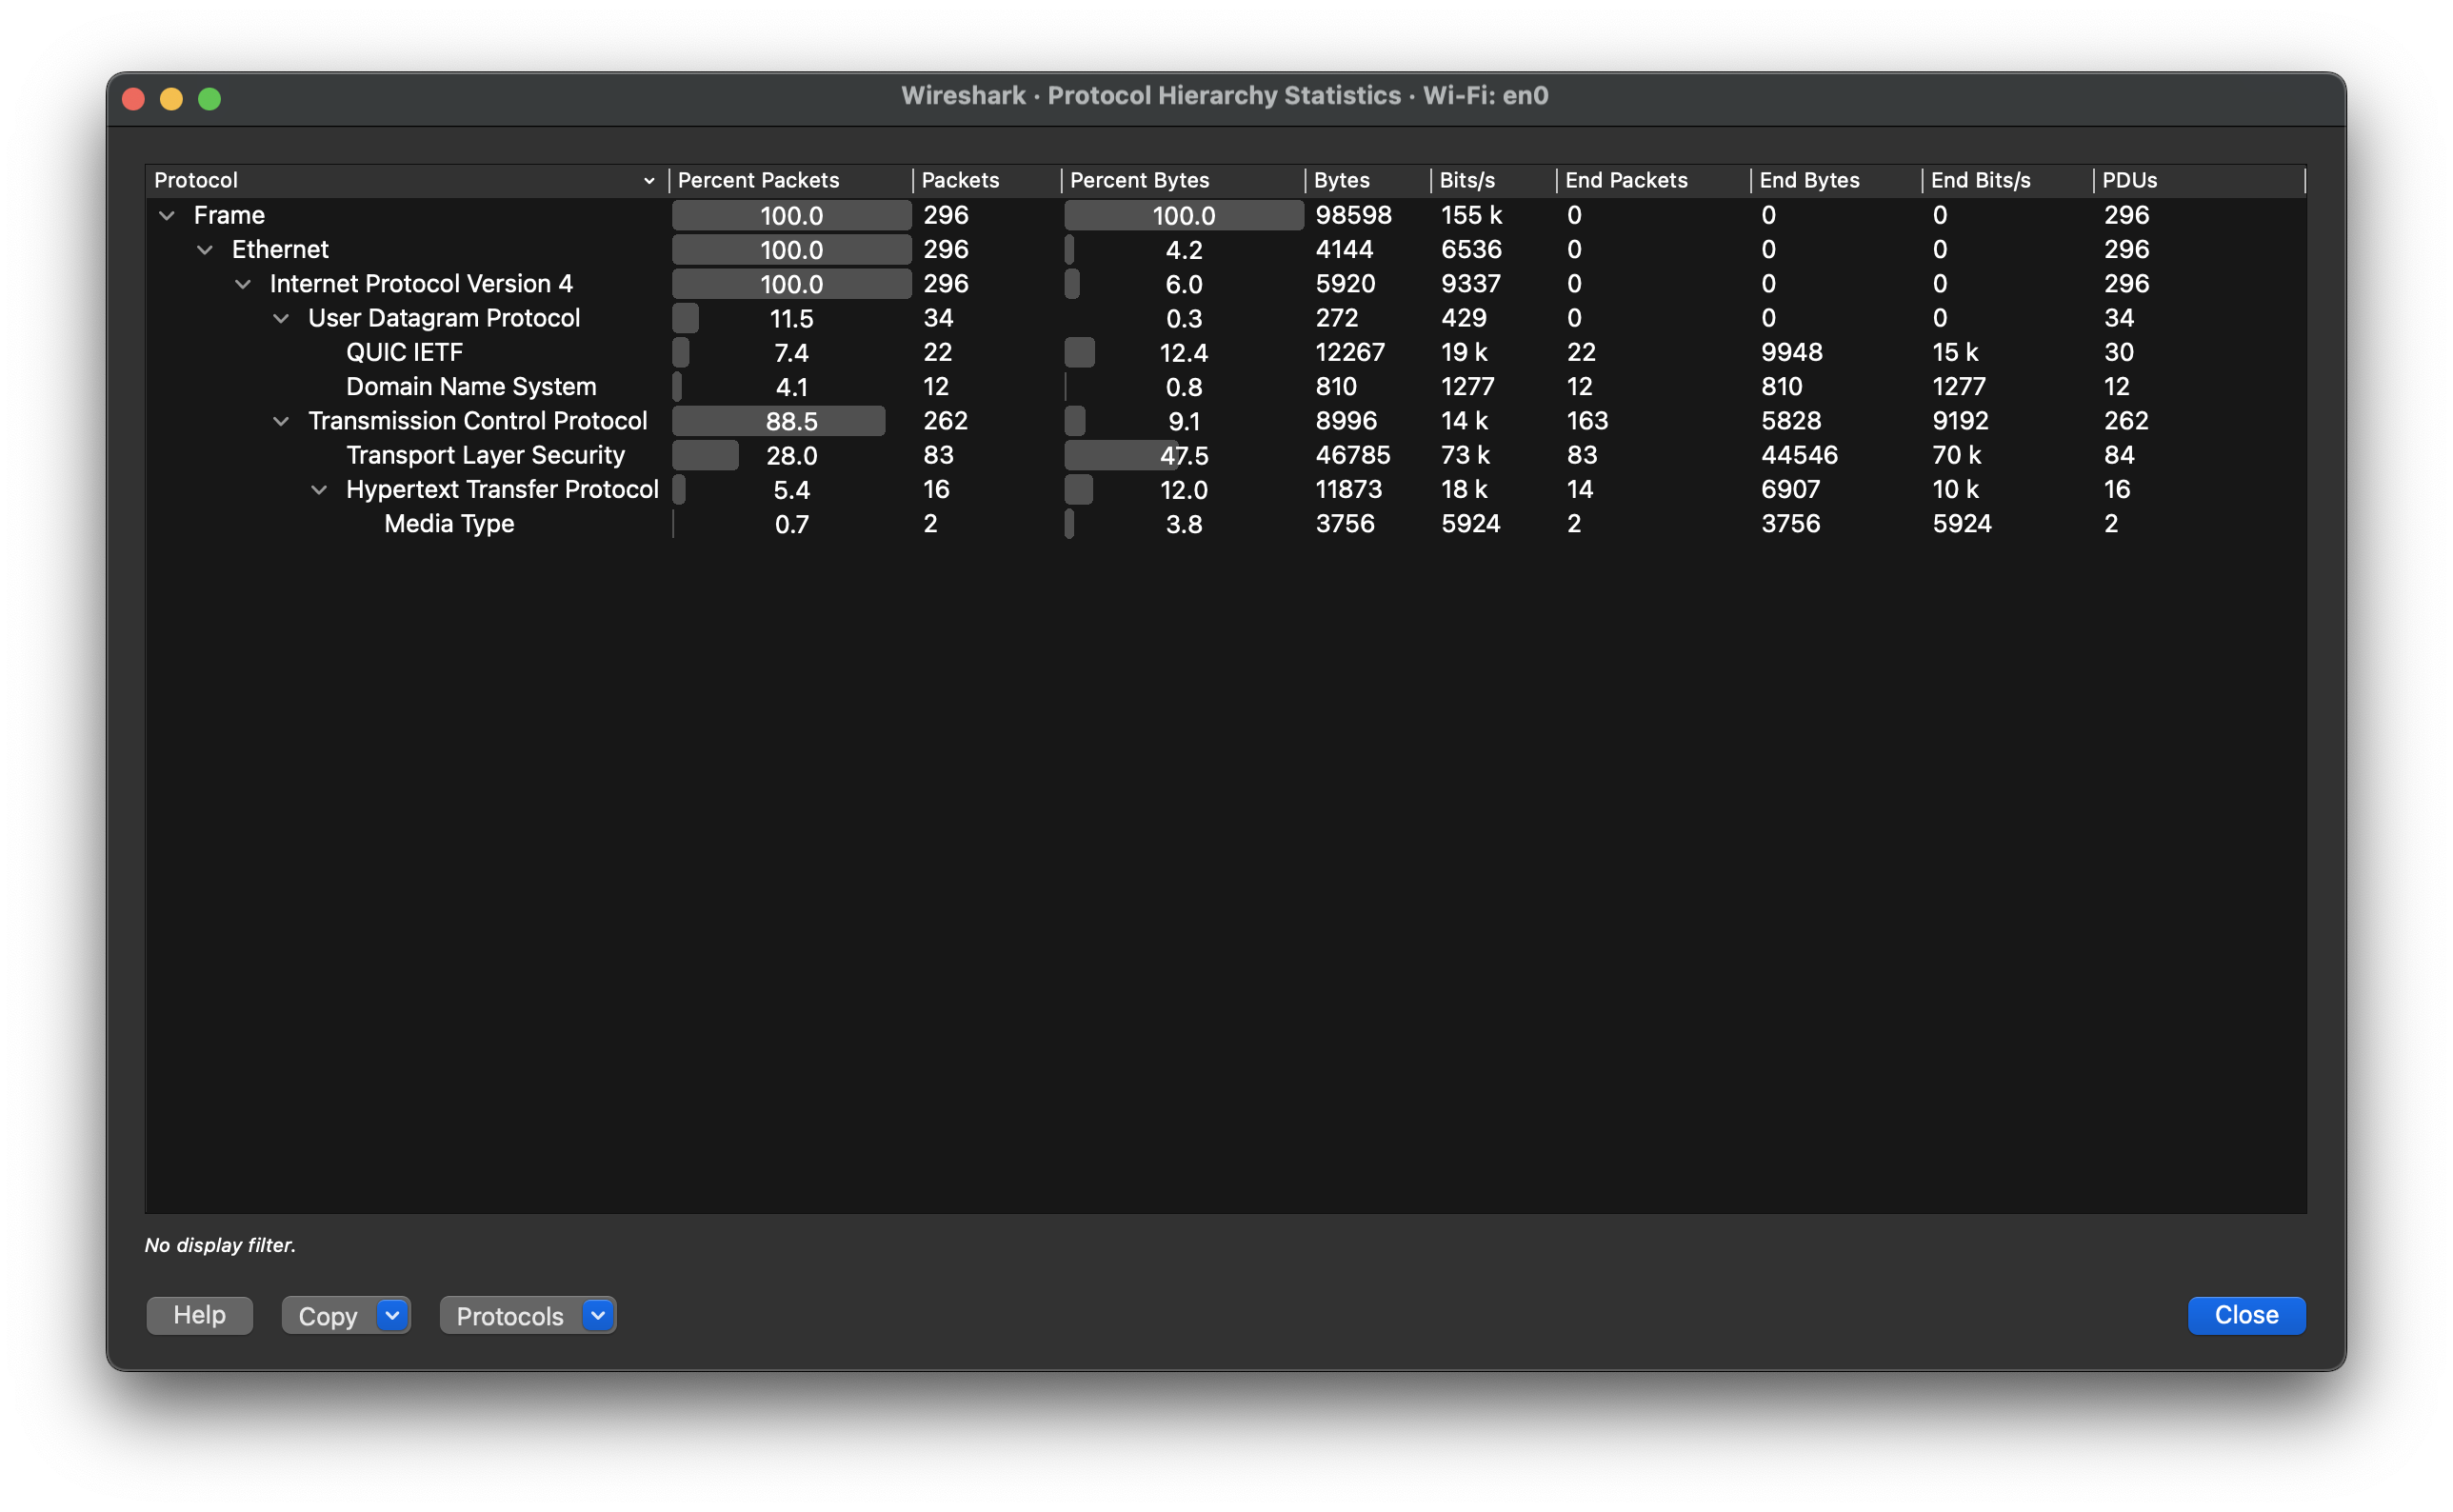
\includegraphics[width=1\textwidth]{figs/2.png}
		
	}
}

\begin{itemize}
   \item   تمامی پکت‌ها از لایه لینک عبور کرده‌اند.
   \item ۱۰۰ درصد بسته‌ها از پروتوکل \lr{IPv4} استفاده کرده‌اند.
   \item حدودا ۸۸ درصد از بسته‌ها از پروتوکل TCP بر بستر \lr{IPv4} استفاده کرده‌اند.
   \item ۱۲ درصد بسته‌ها از پروتوکل UDP بر بسته \lr{IPv4} استفاده کرده‌اند.
\end{itemize}

\subsubsection*{سوال 2.}

{
	\centering{
		
		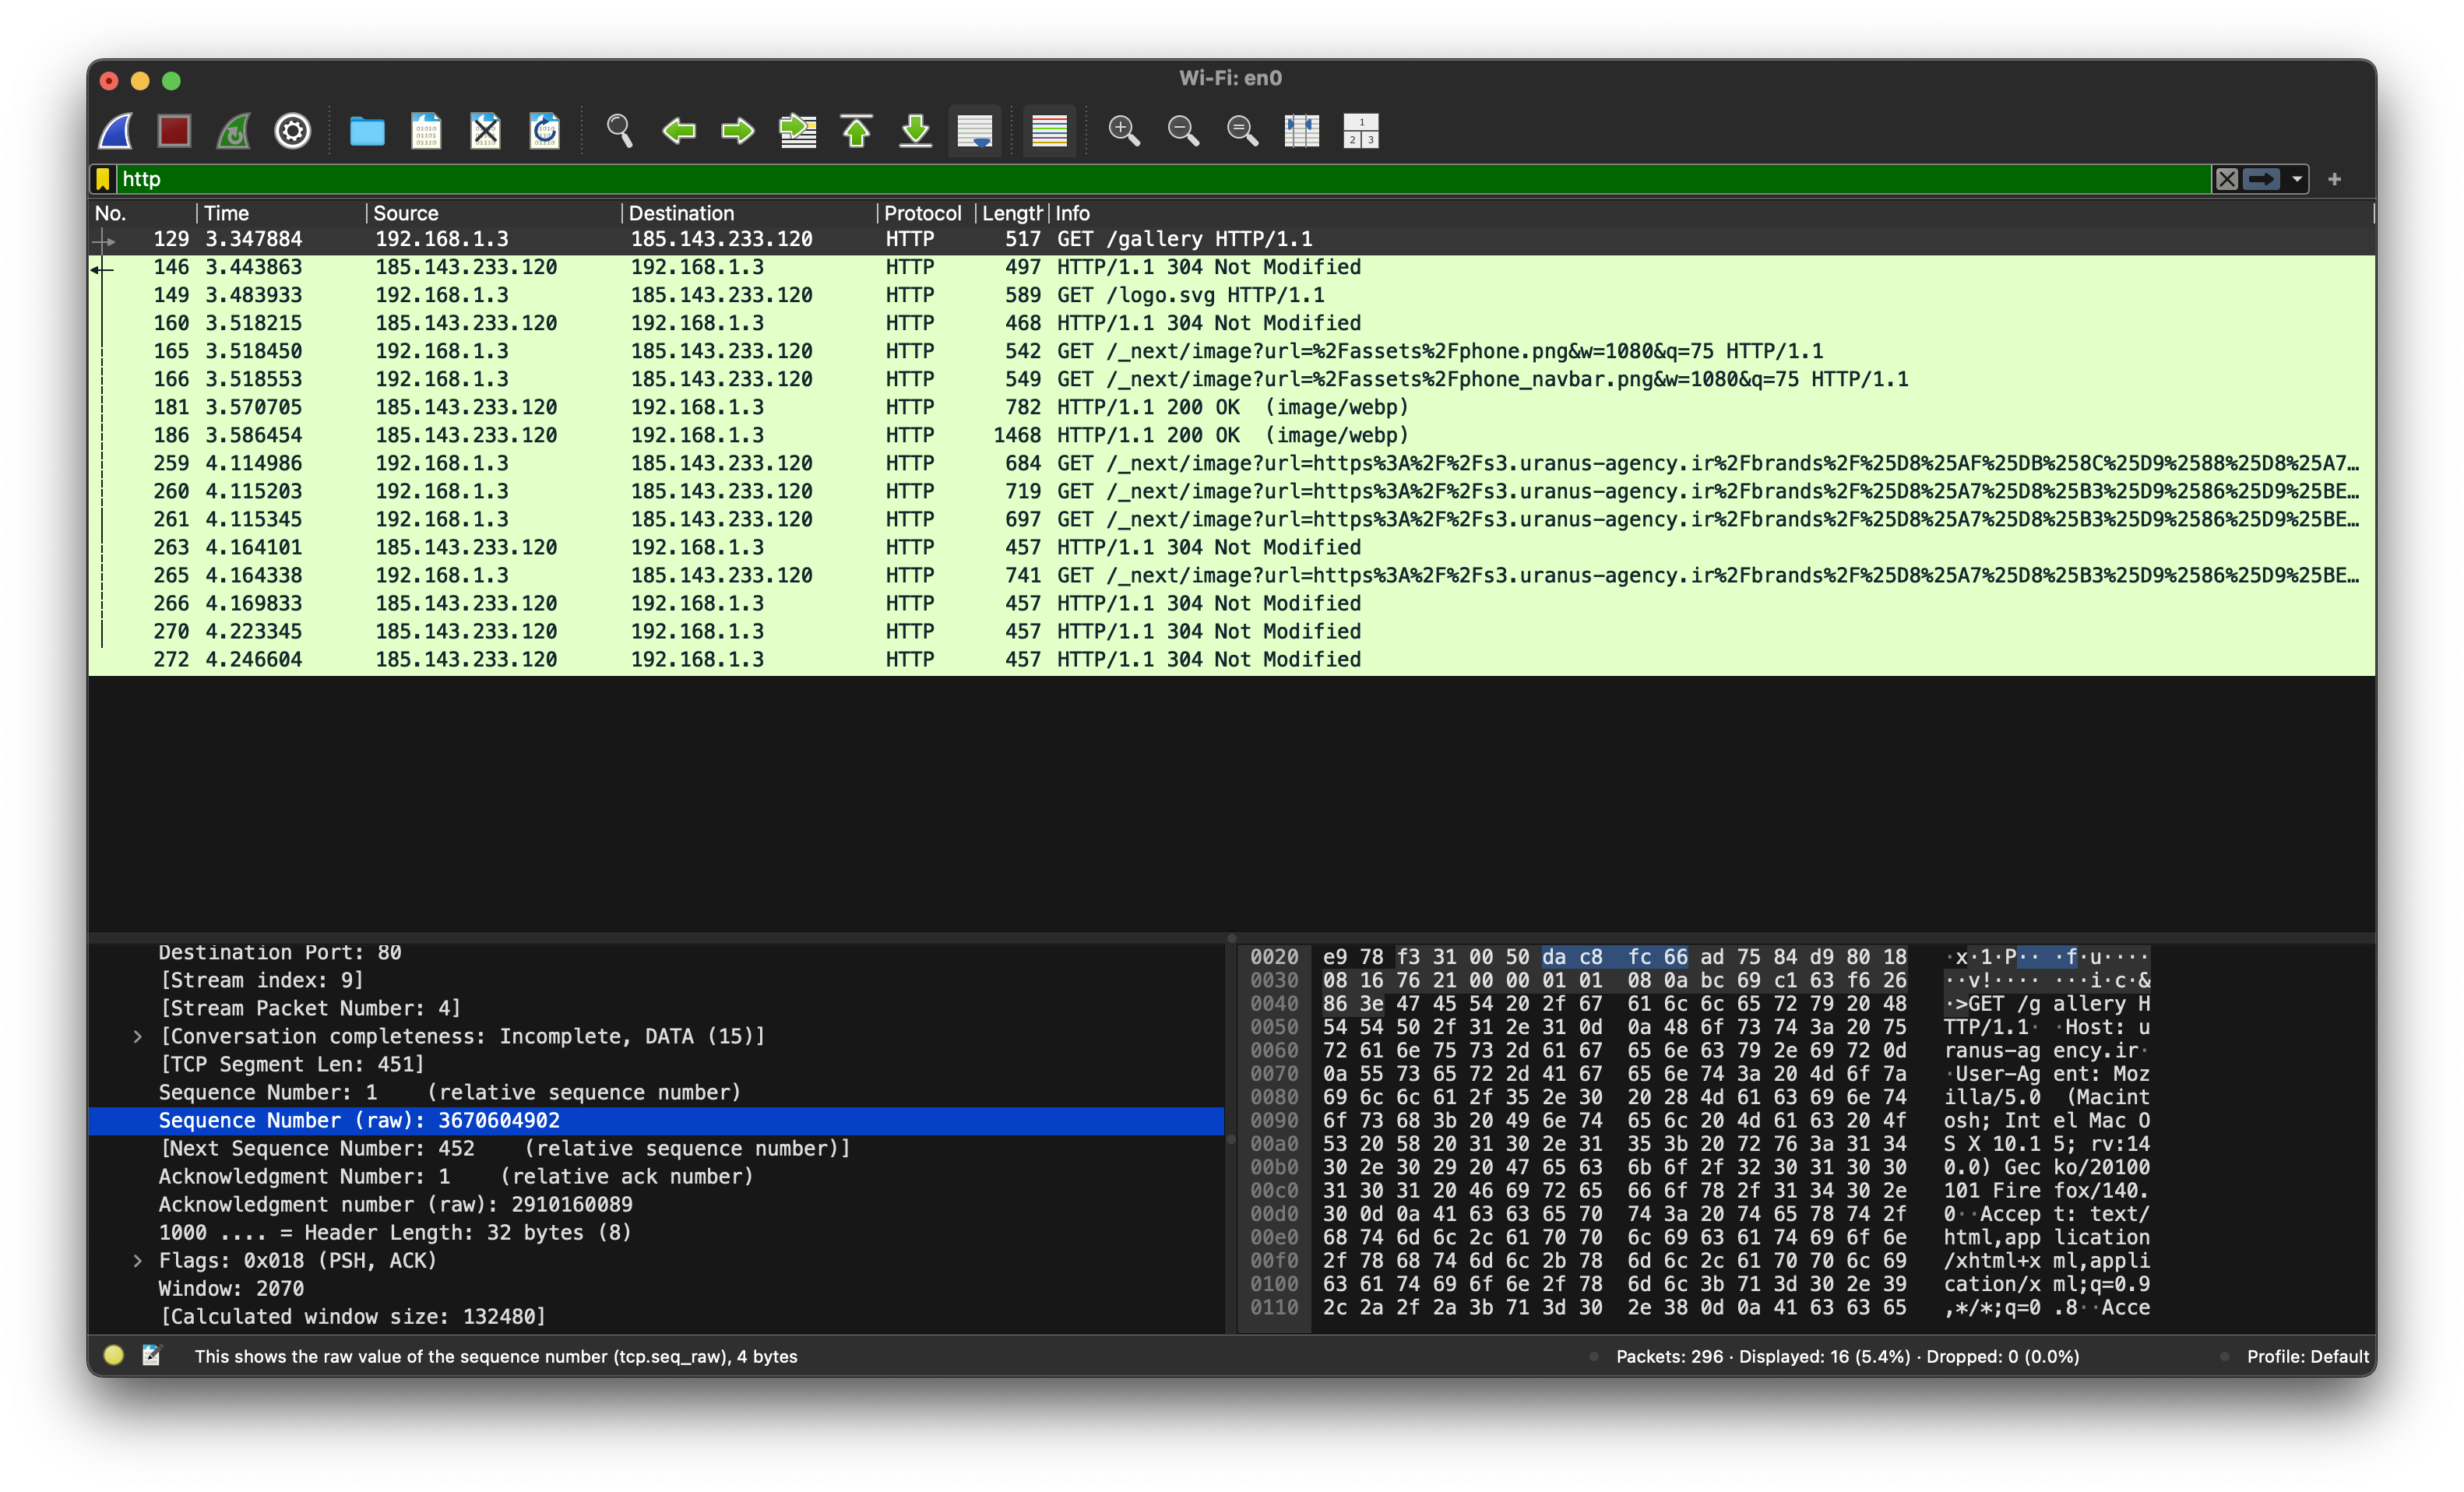
\includegraphics[width=1\textwidth]{figs/3.png}
		
	}
}

بسته شماره ۱۲۹ به مقصد رسیده و میزبان در بسته ۱۴۶ پاسخ با کد ۳۰۰ داده است یعنی این عکس تغییر نکرده و باید از کش خوانده شود. اختلاف زمانی این دو بسته در ستون دوم مشخص است.

می‌توان بسته ‍۱۶۵ و ۱۸۱ را هم مشاهده کرد که درخواست عکس را دارد و پاسخ 
\lr{http ok}
را دریافت کرده است.


{
	\centering{
		
		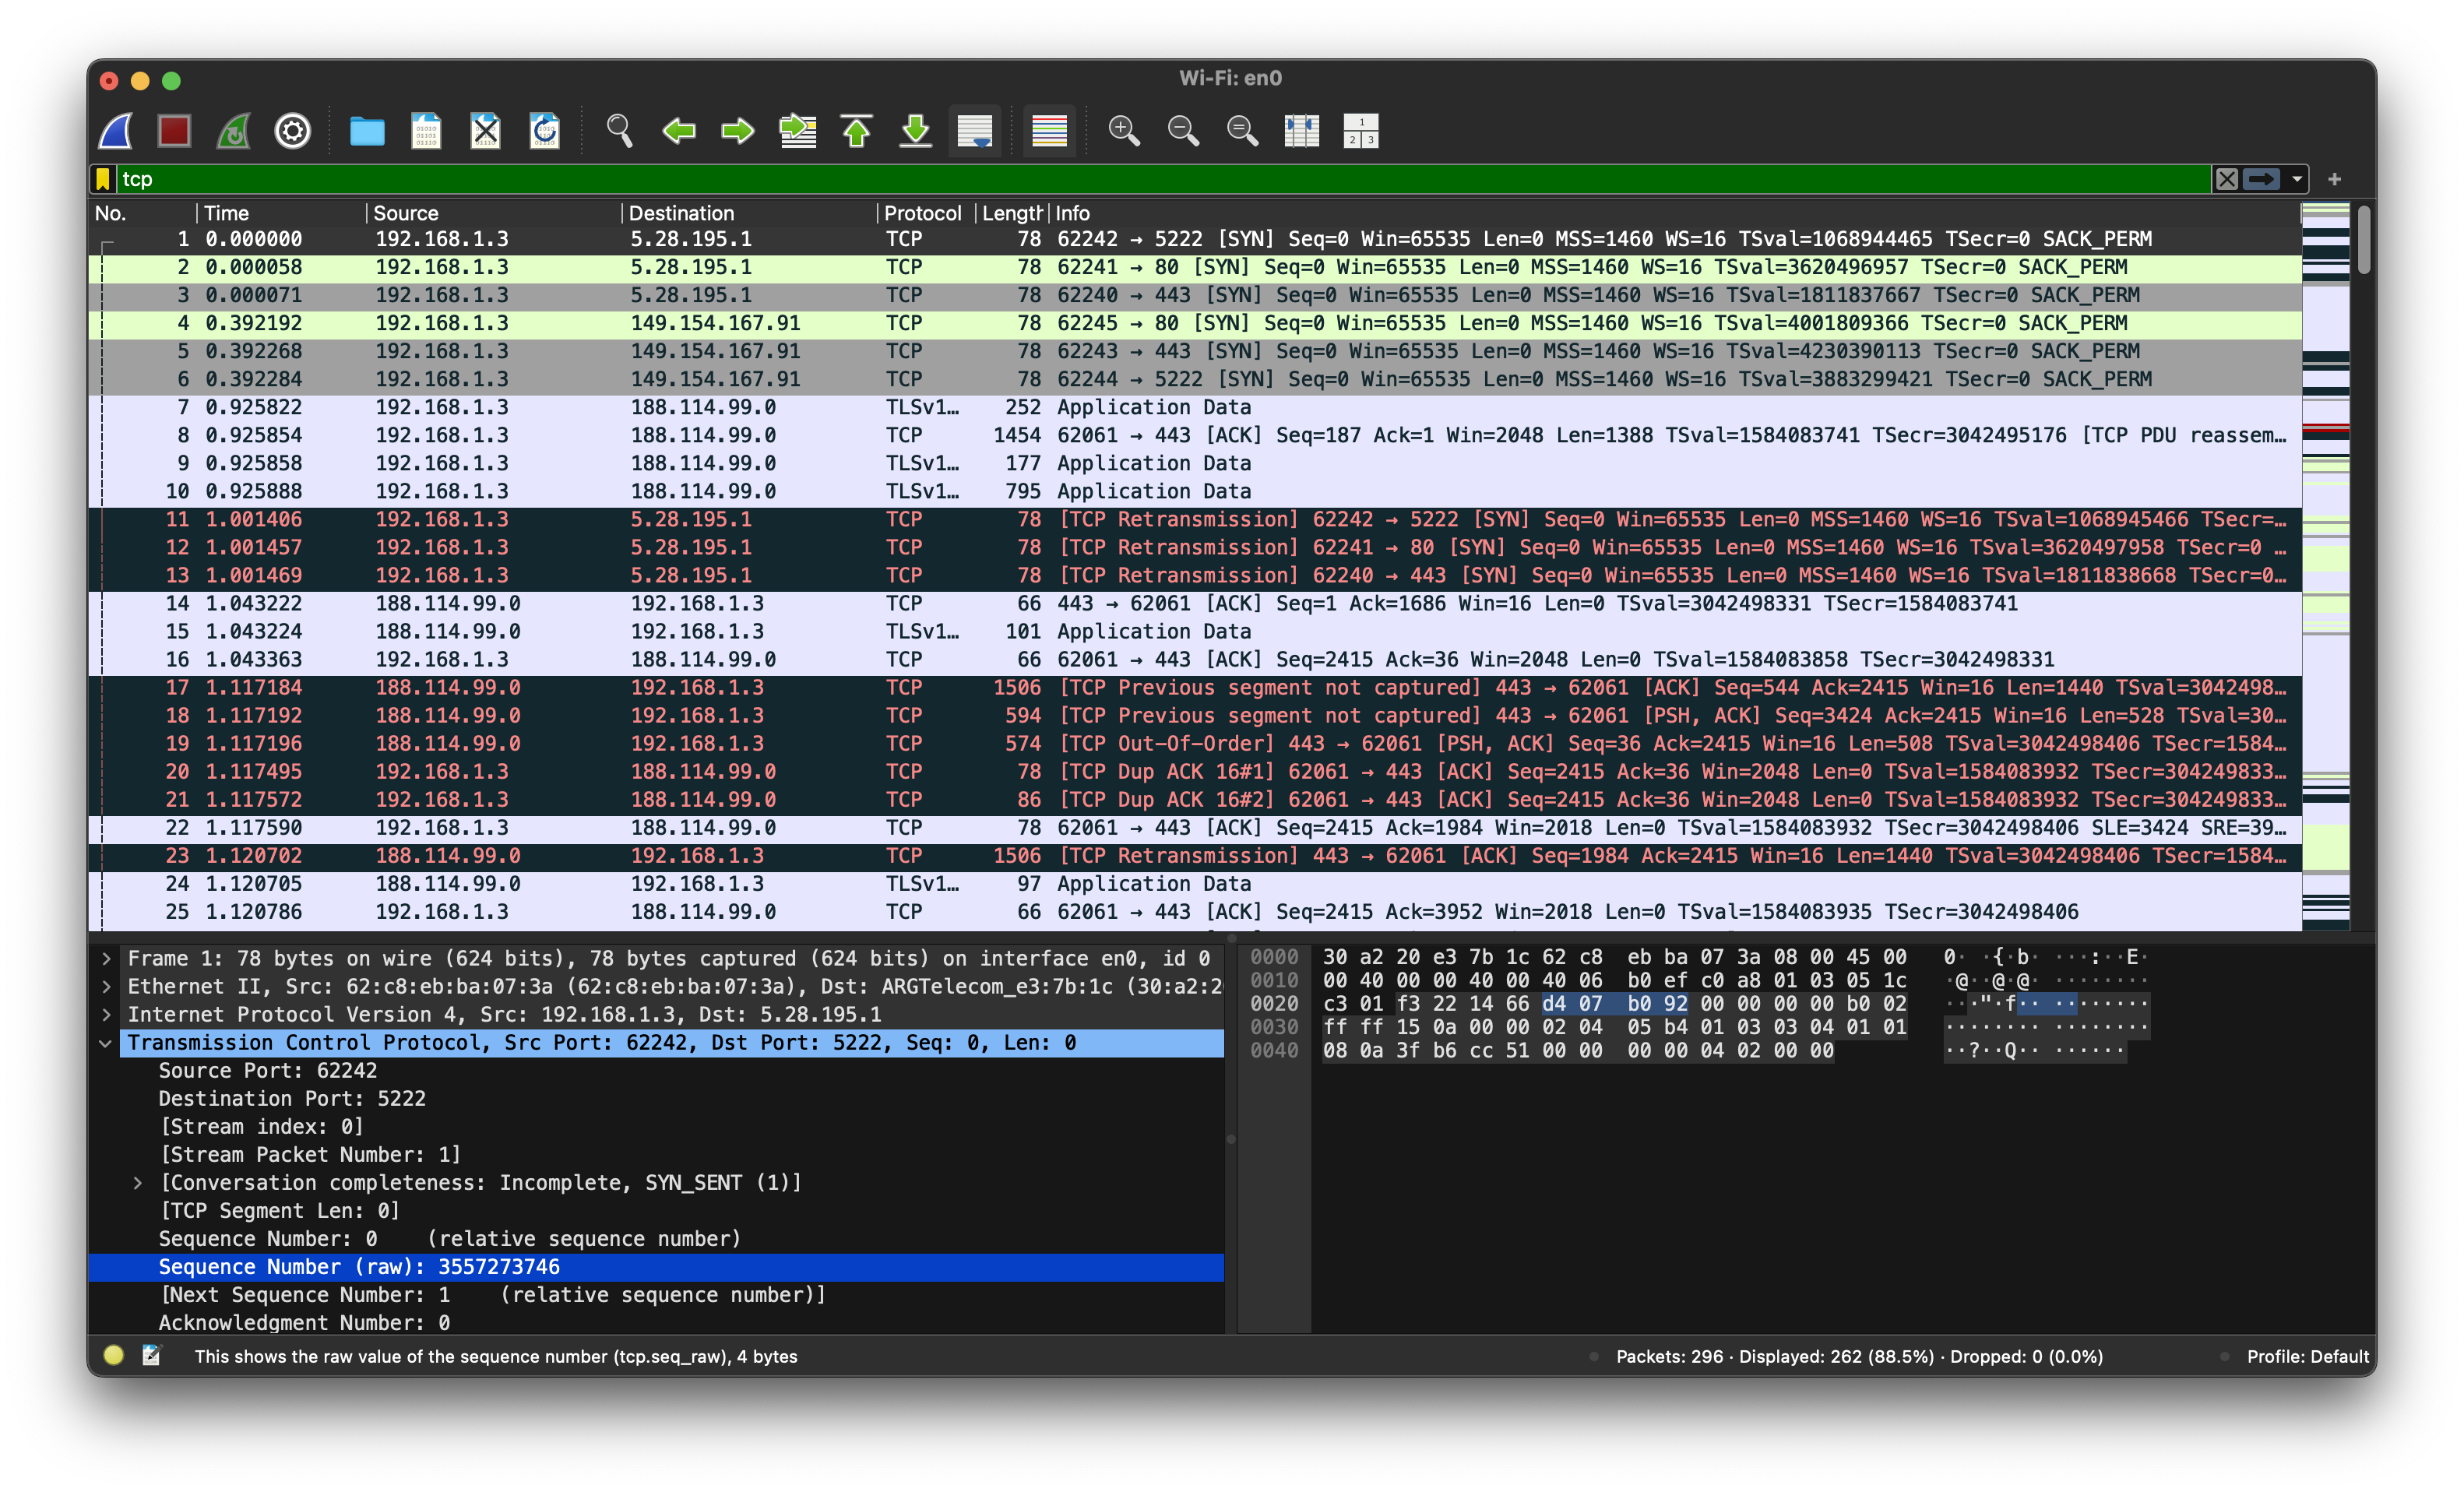
\includegraphics[width=1\textwidth]{figs/4.png}
		
	}
}

همچنین شماره ترتیب مطلق اولین ارتباط TCP برابر است با 
3557273746.

\subsubsection*{سوال 3.}

{
    \centering{
        
        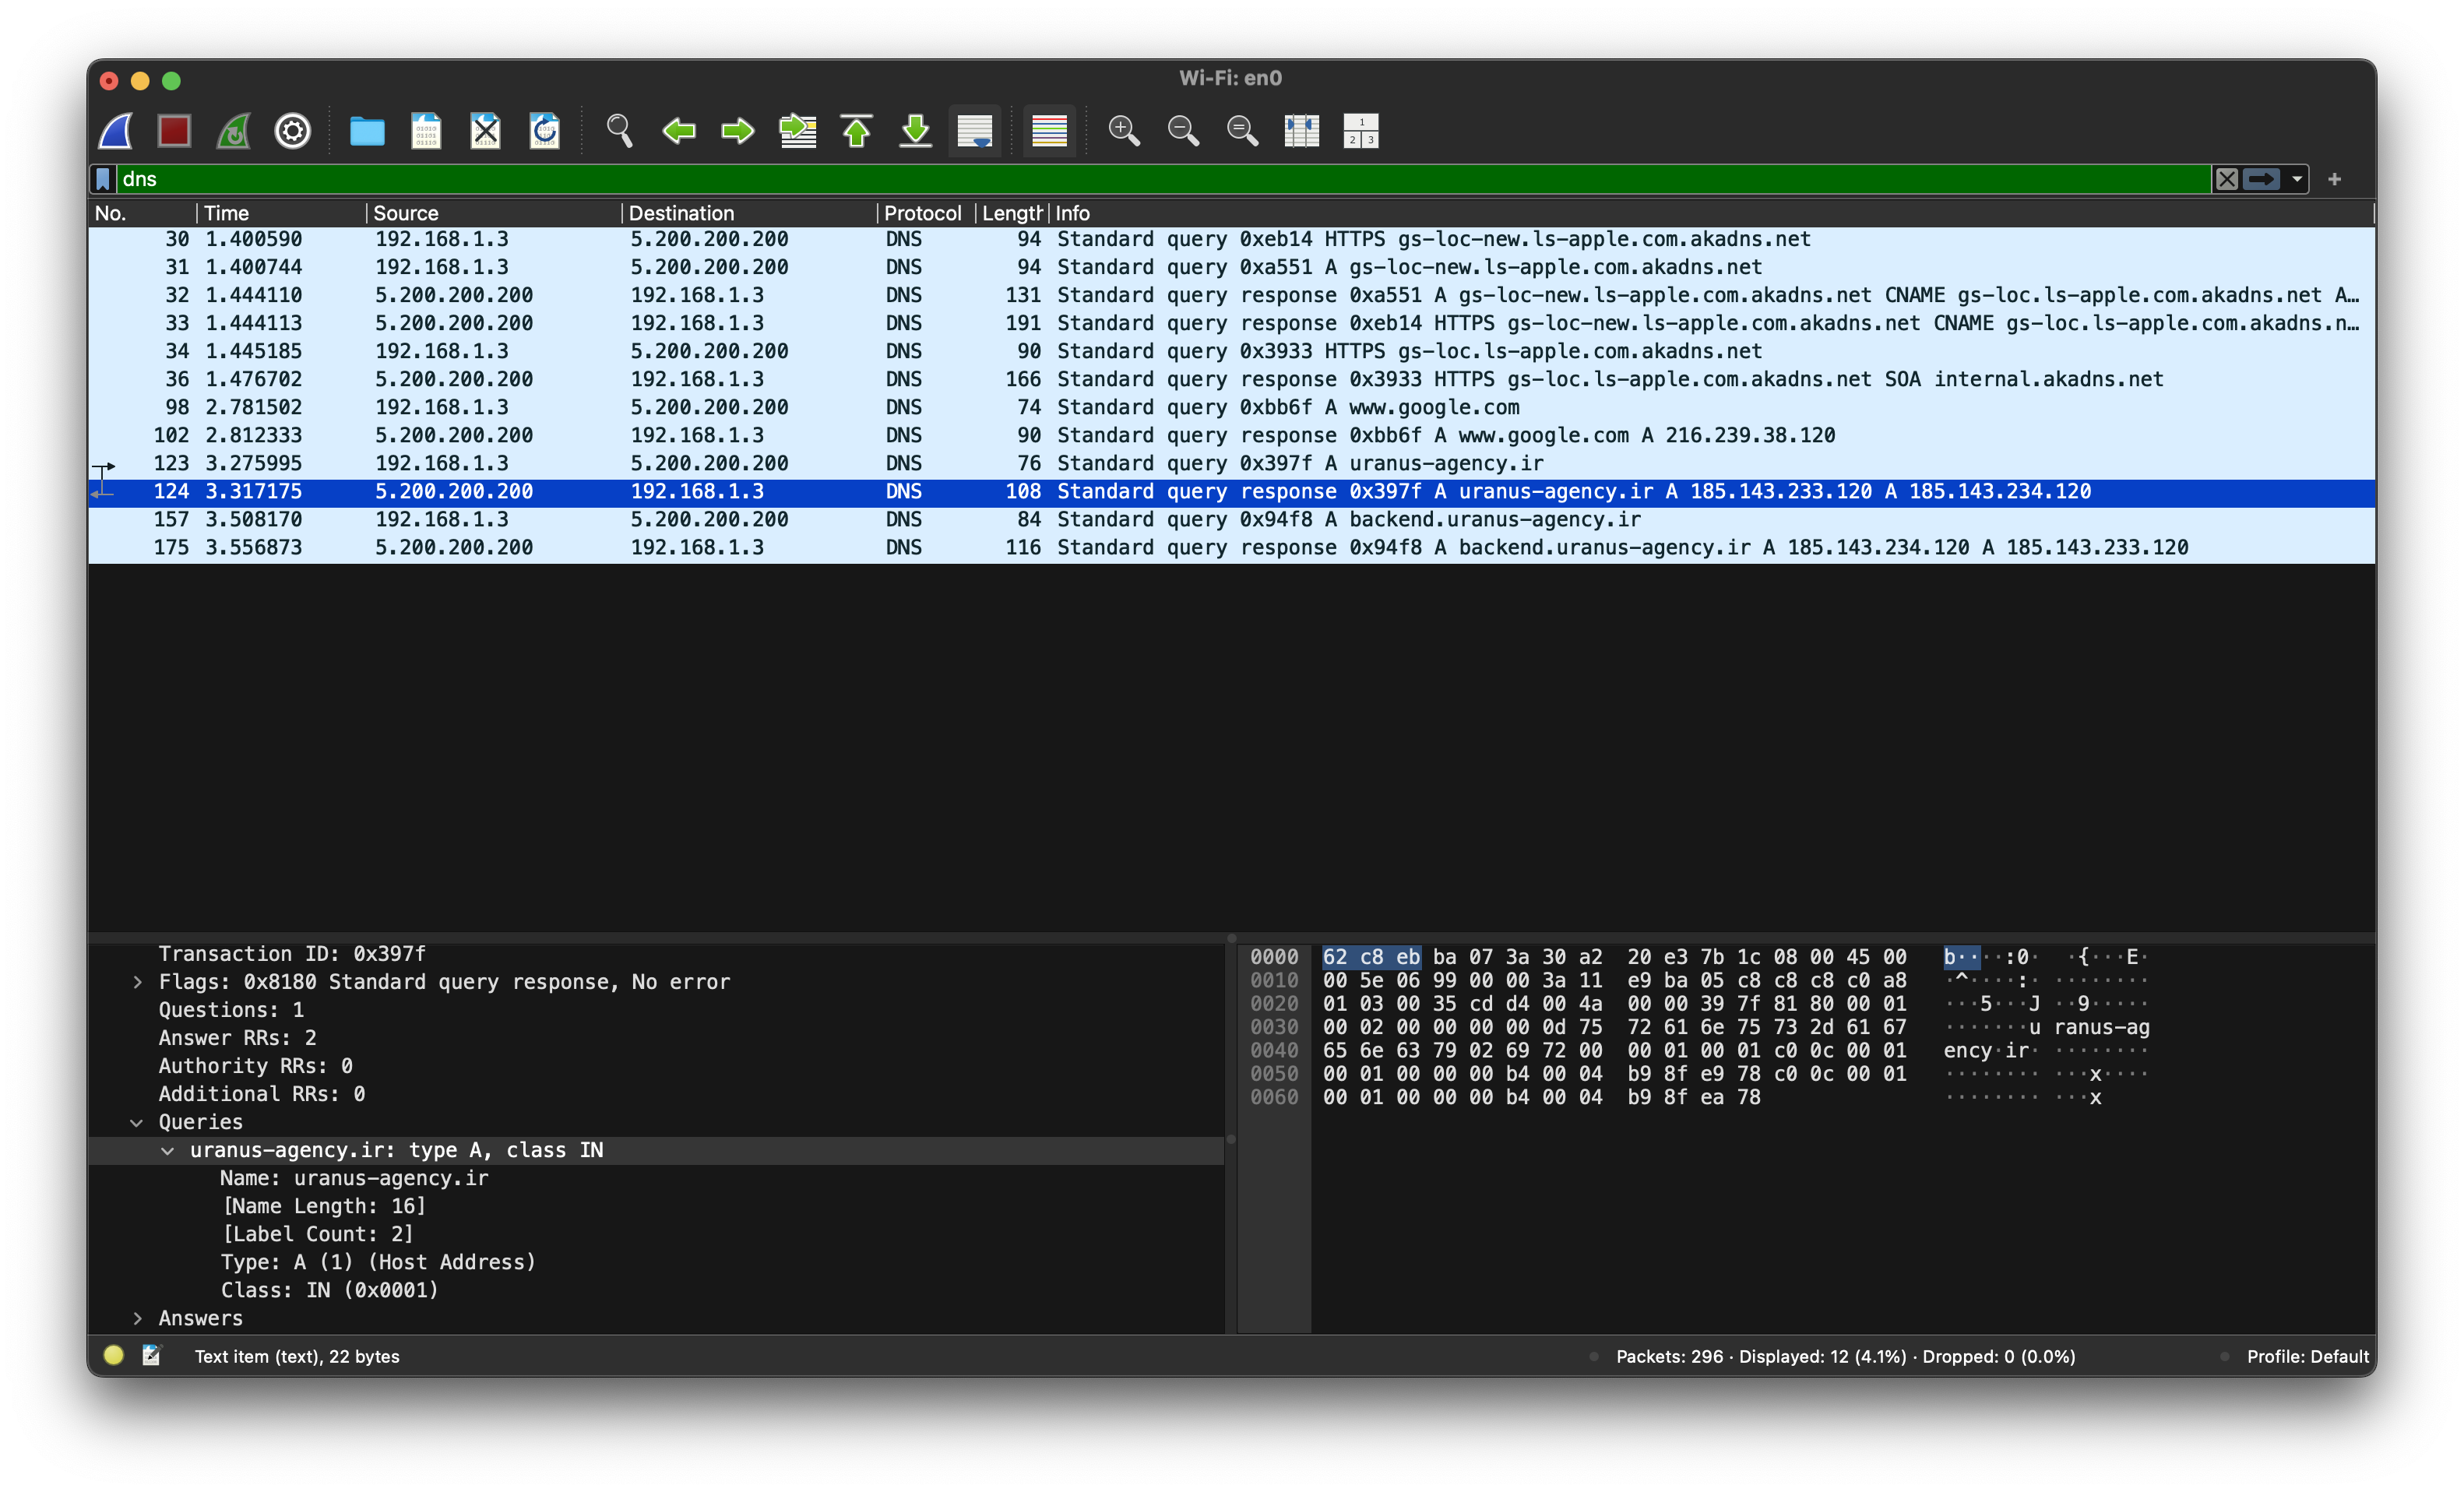
\includegraphics[width=1\textwidth]{figs/5.png}
        
    }
}

کوئری‌های درخواست DNS از نوع
\lr{Standard DNS Query}
هستند.

کوئری و پاسخ DNS هر دو از یک نوع هستند با این تفاوت که در پاسخ،
فلگ پاسخ فعال است و پاسخ را هم به همراه دارد.

همچنین نوع رکورد درخواست شده از نوع A است.

{
    \centering{
        
        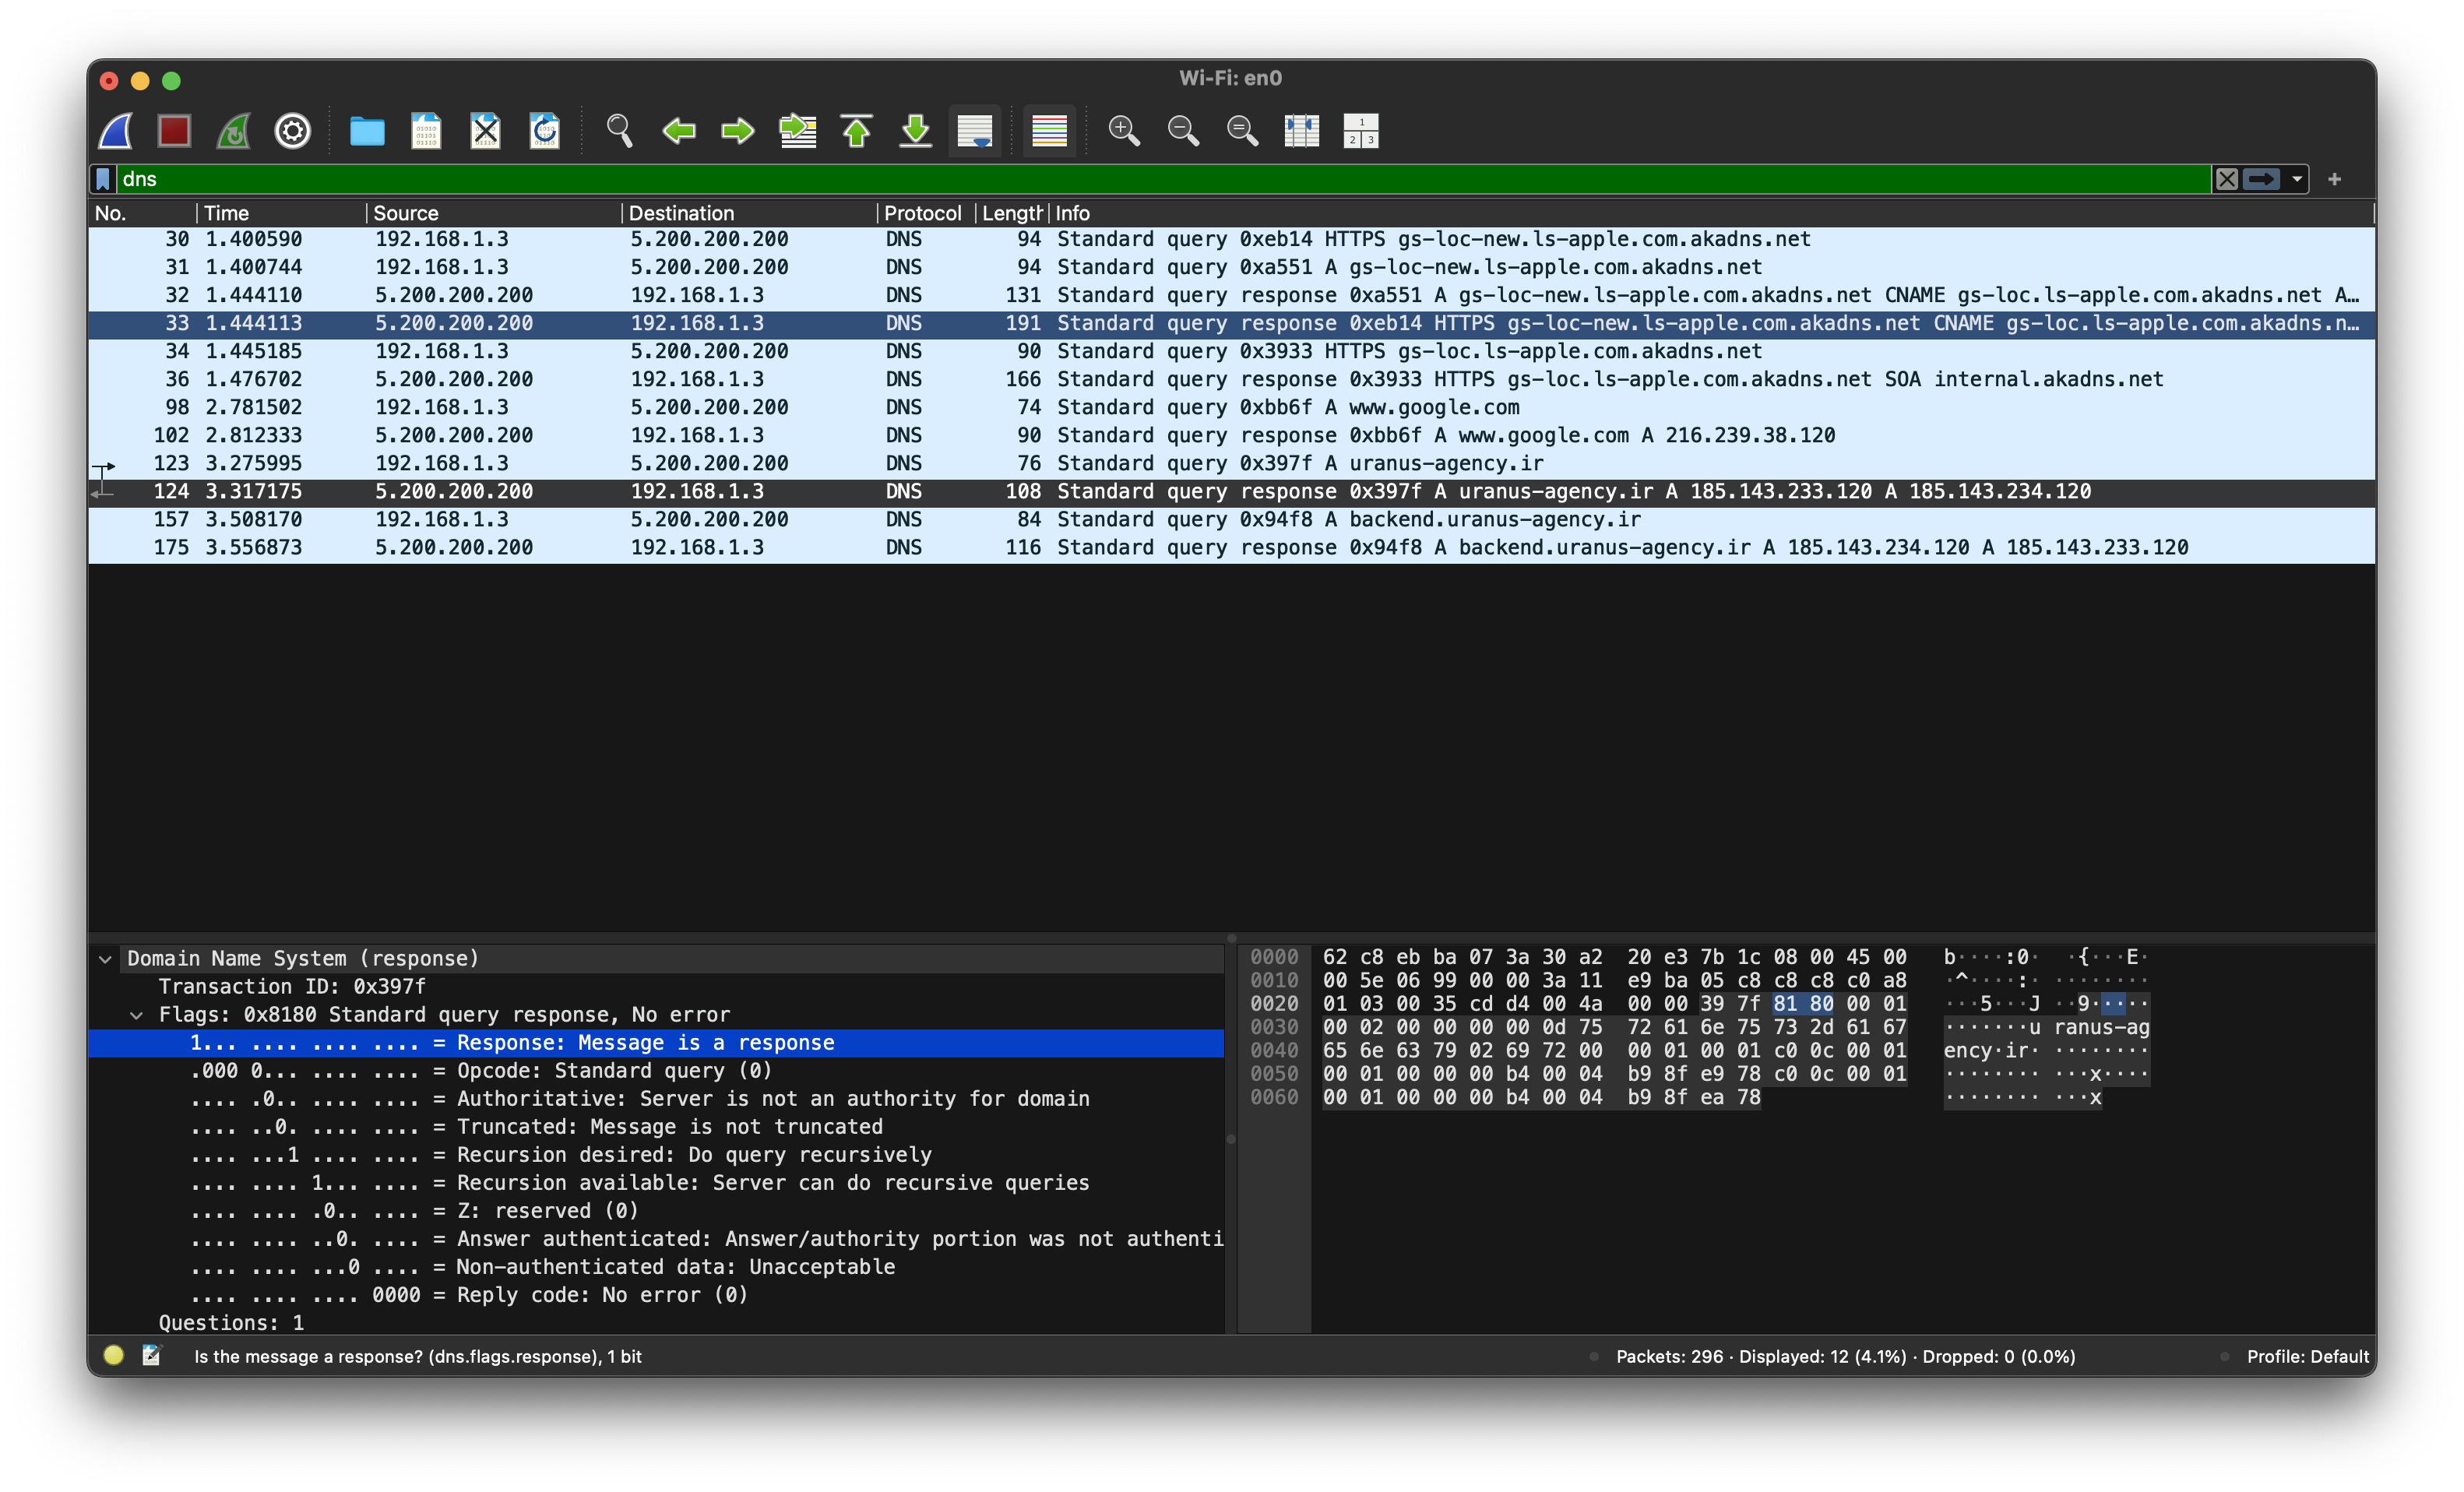
\includegraphics[width=1\textwidth]{figs/6.png}
        
    }
}

در شکل فوق مشخص است که فلگ پاسخ برابر ۱ شده است و نوع رکود هم نوشته شده است و برابر A است.

\subsubsection*{سوال 4.}

برای ذخیره کردن عکس‌ها، پکت درخواست آن عکس را سلکت کرده و سپه و سپس مشابه تصویر زیر عمل می‌کنیم:

{
    \centering{
        
        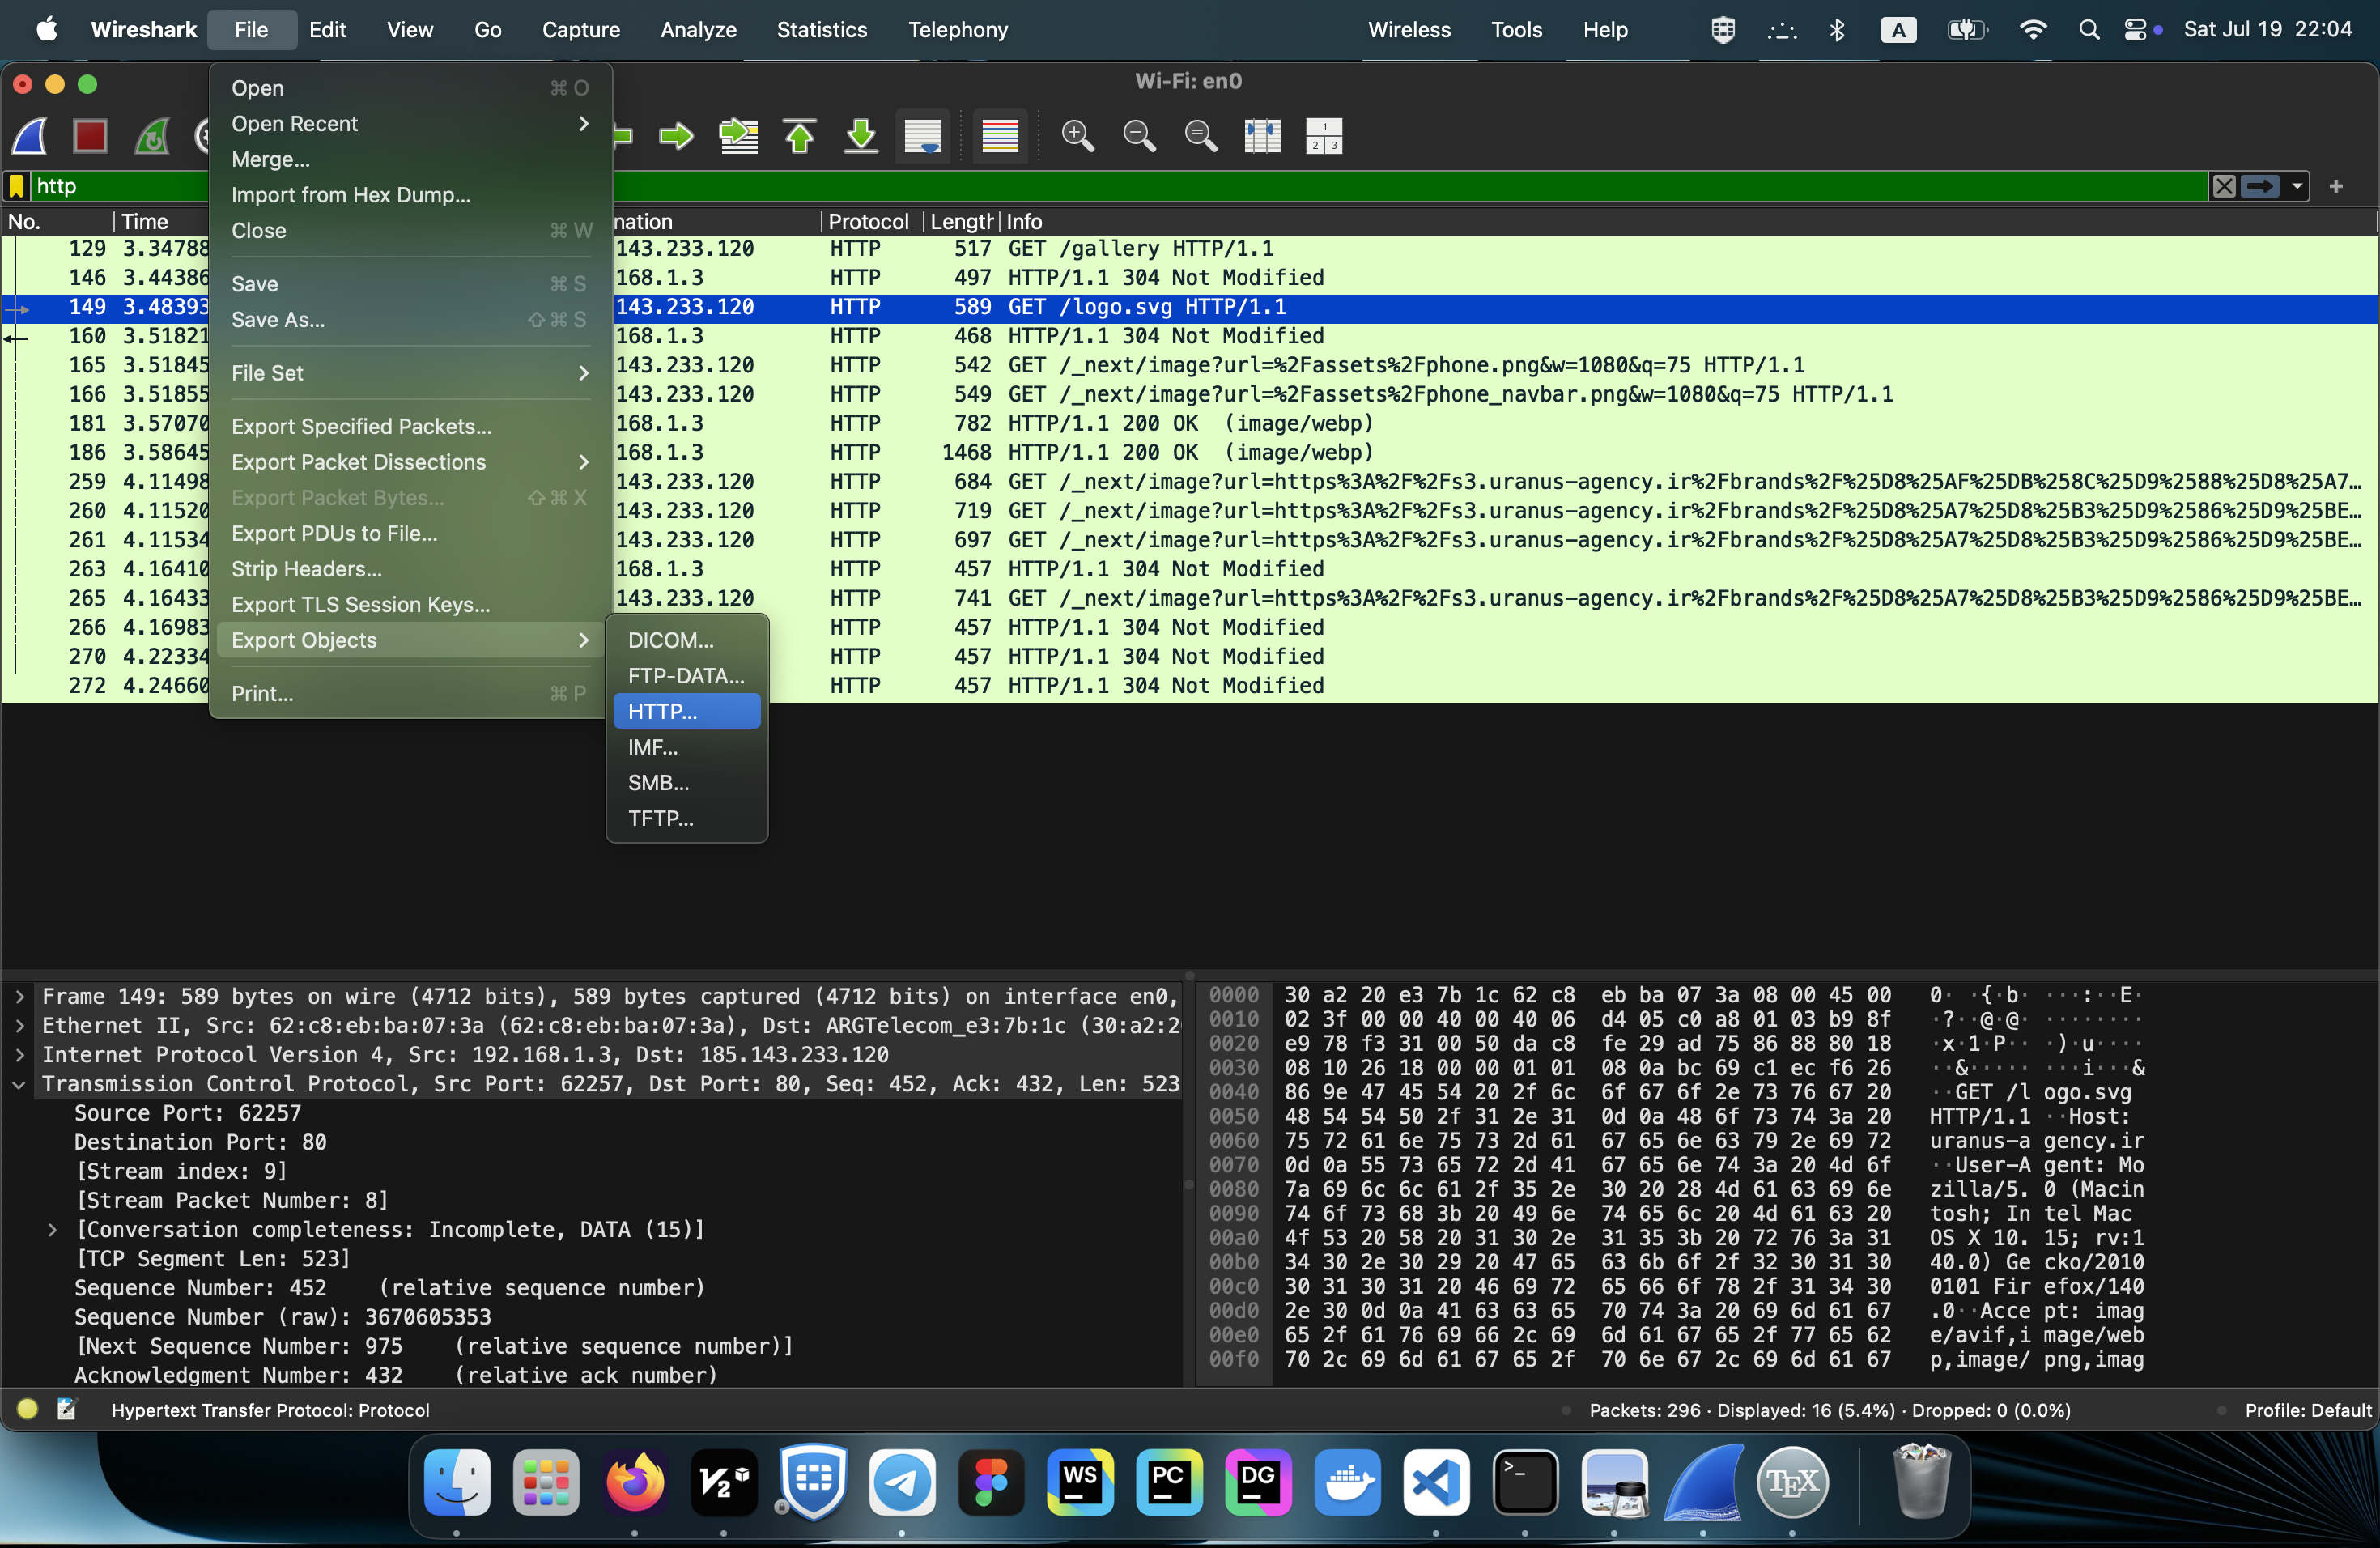
\includegraphics[width=0.9\textwidth]{figs/7.png}
        
    }
}